\begin{homeworkProblem}[HAPI simulator exercises]
\label{sec:hapi}

\begin{homeworkSection}{Exercise 1}

\subsubsection{LL bound}
\begin{tabular}{l|l|l}
	& $C_i$ & $T_i$ \\
	\hline
	$\tau_1$ & 2,5 & 5 \\
	\hline
	$\tau_2$ & 4 & 9 \\
\end{tabular}


For the LL-bound check, we need to know the least upperbound for this schedule. Since we have two tasks, equation \ref{eq:lub} has to be calculated for two tasks.

\begin{equation} \label{eq:lub}
\begin{split}
U_{lub} &= 2*(2^{1/n}-1)\\
		&= 0.828
\end{split}
\end{equation}

Then, for the bound check we need the utilization factor. If this value is smaller than the $U_{lub}$, 

\begin{equation} \label{eq:util}
\begin{split}
U 	& = \sum_{i=1}^2 \frac{C_i}{T_i} \\
	& = \frac{2,5}{5} + \frac{4}{9}\\
	& = \frac{17}{18}\\
	& = 0.944....\\
\end{split}
\end{equation}

This is clearly greater than 0.828, therefore the schedule is not feasible according to the LL bound.

\subsubsection{HB bound}
So then for the schedule to be feasible according to the HB bound, the result of equation \ref{eq:util_hb}.

\begin{equation} \label{eq:util_hb}
\begin{split}
\prod_{i=1}^{2} (U_{i} + 1) & = 1\frac{1}{2} * 1\frac{4}{9} \\
		& = \frac{13}{6}	
\end{split} 	
\end{equation} 

This is larger than 2, therefore the schedule is not feasible according to the HB bound.

\subsubsection{Wort-case response time}

Then for the worst-case response time. First for $\tau_1$:

\begin{equation} \label{eq:e1_wrc1}
\begin{split}
R_1^0 & = C_1 \\
			& = 2.5 
\end{split}
\end{equation}

And for $\tau_2$:

\begin{equation} \label{eq:e1_wrc2}
\begin{split}
R_2^0 	& = C_2 \\
		& = 4	\\ 
R_2^1 	& = I_2^0 + C_2 \\
		& = \frac{4}{5}*2.5 + 4\\
		& = 6 \\
R_2^2 	& = I_2^1 + C_2 \\
		& = \frac{6}{5}*2.5 + 4 \\
		& = 7 \\
R_2^3	& = I_2^2 + C_2 \\
		& = \frac{7}{5}*2.5 + 4 \\
		& = 8 \\ 
R_2^4	& = I_2^3 + C_2 \\
		& = \frac{8}{5}*2.5 + 4 \\
		& = 8
\end{split}
\end{equation}
\end{homeworkSection}

Thus, the worst-case reponsetimes are 2.5 for $R_1$ and 8 for $R_1$. Both are within the deadlines and therefore the schedule should be feasible.

\subsubsection{HAPI implementation}

The script is edited and now looks like this:

\CCscript{rma1}{The HAPI script for ex1}

The simulation yields the result and matching waveforms given below. Interest is that the worst-case response time for $\tau_1$ is 2 ns according to the simulator. 
Inspection of the waveforms shows indeed a calculation time of 2 ns instead of 2.5. Probably, the value is rounded early on.

\TXTscript{hapi_out_1}{HAPI output}

\begin{figure}[h]
	\label{fig:hapi_wave_1}
	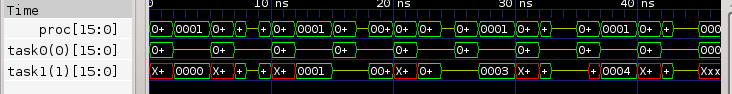
\includegraphics[width=480px]{figures/hapi_wave_1.png}
	\caption{Waveforms of processor and tasks}
\end{figure}

\newpage

\begin{homeworkSection}{Exercise 2}
\begin{tabular}{l|l|l|l}
	& $C_i$ & $T_i$ & Priority \\
	\hline
	$\tau_1$ & 30 & 50 & lower \\
	\hline
	$\tau_2$ & 30 & 100 & higher \\
\end{tabular}

\subsubsection{Wort-case response time}

For $\tau_1$, which immediately interrupted by $\tau_2$, the worst-case response time is $30+30=60$. This means a violation of the deadline. 
For $\tau_2$ the the worst-case response time is 30, as it is handled immediately.
Because of the deadline violation, the schedule is not feasible.

\subsubsection{HAPI implementation}

The script is edited and now looks like this:

\CCscript{spp2}{The HAPI script for ex1}

Despite the bound, it is a feasible schedule.
\TXTscript{hapi_out_2}{HAPI output}

\begin{figure}[h]
	\label{fig:hapi_wave_2}
	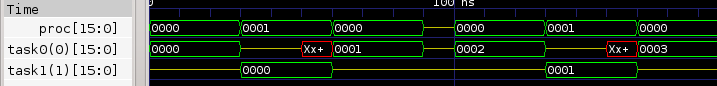
\includegraphics[width=480px]{figures/hapi_wave_2.png}
	\caption{Waveforms of processor and tasks}
\end{figure}

\subsubsection{Questions}
The task with the higher priority has an offset that is exactly equal to the execution time of lower prioritized task. 
Since that task arrives first, the first execution is handled without interrupts. 
Besides, the task periods are harmonic and the utilization factor is lower than 100\%. This means that with the proper offset, the schedule is feasible if the utilization factor is $\leq 100\%$.

The task set is infeasible and gives worst-case response time if $0 \leq offset_{R_2} modulo 50 \leq 29$

\end{homeworkSection}

\end{homeworkProblem} 